% Shawn Waldon - This is my PRP paper.


\documentclass{article} % is article right?

\usepackage{graphicx}
\usepackage{caption}
\usepackage{subcaption}

\begin{document}
% Just working on learning LaTeX
\title{SketchBio: A Scientist's 3D Interface for Molecular Modeling and Animation}
\author{Shawn Waldon\\Department of Computer Science\\
			UNC Chapel Hill\\\texttt{swaldon@cs.unc.edu}}
\date{\today}
\maketitle

\begin{abstract}
Molecular modeling for animation is typically done with programs that are difficult to learn and use, controlled by a keyboard and 2D mouse.  Discussions among collaborators are typically done with 2D whiteboard sketches.  Some scientists hire professional computer programmers and/or animators and work with them to create 3D models and animations.  SketchBio is a new application that uses a pair of 6-degree-of-freedom trackers to help scientists more easily assemble and animate 3D models of molecular structures.  To maximize productivity, SketchBio avoids making the user wait unnecessarily.  Operations that can negatively impact the interactivity of the application include collision detection and rendering.  Rendering speed can be significantly improved by substituting simpler geometric models for the actual polygonal mesh wherever size and viewpoint permit.  Collision detection is one of the most expensive operations in systems with many molecules, so SketchBio implements (1) “pose mode” physics where only objects that are directly interacted with move or are tested for collisions and (2) an order of magnitude reduction in the number of tests needed within ‘crystal-by-example' objects due to the predictable relative positions of objects.  Another way to decrease the users' active waiting time is by moving non-immediate tasks that will cause waits to background threads or processes.  SketchBio also leverages existing tools to perform many operations (loading molecules, generating surfaces for molecules, and high quality rendering).  These features (along with a rich user interface with biologically driven operations) provide a thinking and design environment that is easy and rapid to use by biologists.

\end{abstract}

\section{Introduction}
SketchBio is a system for understanding subcellular biology through the building of complex 3D macromolecular structures, and animating the structures over time.   The modeling, simulation, and rendering of these hypothetical situations currently involves accessing and using a number of tools and databases (PDB, UCSF Chimera, Blender, NAMD, and MicroscopeSimulator) and then converting files and data to pass between tools.  It also involves manual placement of 3D objects, which is currently done using clunky 2D input devices and by-eye detection and avoidance of collisions.  Some scientists hire professional computer programmers or animators to create 3D models and animations for them due to the high learning curve of typical modeling and animations, adding an additional communication barrier to the process.  As a result, it often takes a team months to produce an acceptable model or animation.  We aim to reduce this to a single person working for hours or days.

The initial driving problem for this project was recently-retired collaborator Susan Lord's desire to construct a protofibril model based on geometric constraints among a set of fibrinogen monomers.  Based on the crystallized structures of fibrin monomers from different species and on only two sets of known interactions \cite{lord2007fibrinogen}, she sought to construct 3D protofibril structures matching those seen in TEM studies.  Over the process of several months, she and her students worked with Resource staff scientist Joe Hsiao to use the UCSF Chimera\cite{pettersen2004ucsf} tool to construct such a model \cite{lordSubmitted}.  Building this model required repeated iteration of hand-placement of two molecules (using multiple 2D mouse interactions), followed by using replication tools to develop candidate models, which were then evaluated against the data.  Lord's use of SketchBio was to construct this protofibril rapidly and semi-automatically, by specifying which location on each fibrin should be in close contact with other molecules and by specifying that the molecules do not overlap.  This same capability will enable generation of other self-symmetric structures such as actin filaments and microtubules.

While developing geometric and mechanical models of the yeast mitotic spindle, we generated several generations of detailed geometric models, from hand-drawn scale models through simplified spring models, to symmetric 3D computer models of the chromosomes and proteins \cite{taylorBookChapter}.  As in the Lord case, each of these generations has required support from an artist, animator, and/or programmer to convert Bloom's conceptual models into geometry for rendering and simulation.  Our program-generated models exhibit more symmetry than the experimental results or conceptual models only because of the difficulty in specifying more complex models that meet the geometric constraints (cohesin loops surrounding four chromatin, no self-intersection or entanglement, etc.).  These programmatic chromosome/protein portions are not currently connected to the semi-symmetric microtubules (both interpolar and kinetochore-attached), which ground the forces to the spindle poles.  Bloom needs SketchBio to support (i) the rapid generation of long coarse-grained interacting polymer chains and their connection to coarse-grained models of symmetric microtubules, (ii) the construction of linked but non-colliding protein-chromosome structures, and (iii) production of simulated fluorescence images from the resulting structures.

Many proteins beyond cohesin and condensin contribute to mitosis, and Kerry Bloom is interested in them all.  His lab is able to fluorescently label both these proteins and chromosome locations, and use multi-color or FRET techniques to determine relative distances and orientations between pairs of proteins.  With accurate localization and tracking for 3D images these techniques provide partial information on the 3D layout of proteins and chromosomes in wild-type and mutant spindles.  Building matching models requires the development of mass-spring-driven semi-automatic layout of proteins within SketchBio.  This will provide a partial set of constraints for the scientist to construct protein-protein and protein-chromosome complexes that match experimental data.  With these enhancements, SketchBio will be widely useful to other researchers for the generation of hypothetical protein-complex structures from partial data.

Scientists are not likely to adopt a tool that requires them to spend a lot of time working on the computer for little payout.  SketchBio aims to minimize and consolidate the time that the scientist spends in front of the computer by running many jobs in the background.  Almost all systems in use in labs have multiple processors and in many cases the background processors can be utilized without interfering with other applications.  SketchBio takes advantage of this in two ways: using background threads to do non-immediate work and calling subprocesses to perform tasks that are already implemented externally.  This allows the scientist to avoid waiting on non-essential background output--to continue working and to perform long-running operations in the background while they work on other things.

\section{Background}
Several other applications targeting similar goals include UCSF Chimera, a tool that SketchBio delegates to internally \cite{pettersen2004ucsf}.  While this application has many features useful to scientists, its complexity makes it difficult to learn, and the mouse and keyboard controls it supports are not optimal for manipulating objects in three dimensions.  The Molecular Control Toolkit is also aimed at molecular modeling, providing an additional user interface for existing tools using gestures to control motions of objects with a Kinect or Leap Motion device \cite{sabirmolecular}.  However, mapping separate inputs to different degrees of freedom for manipulation usually decreases the user's performance\cite{bowman20043d} and the Molecular Control Toolkit maps a separate gesture to each degree of freedom.  Another tool aimed at simplifying the creation of molecular animations, PresentaBALL uses an interactive web interface to an existing molecular modeling tool \cite{nickelspresentaball}.  This allows widespread use but does nothing to assist in the difficult problem of placing things in 6 degrees of freedom.

A common bottleneck in interactive modeling and animation applications is the speed of rendering a complex scene.  A key technique in improving the rendering speed of an application is reducing the complexity of the objects that are drawn.  This is done by replacing objects with imposters have fewer polygons but result in the same or a very similar result being rendered.  Imposters can be difficult to notice, especially if they are far from the camera and the resulting screen area is small.  One type of imposter is a simplified version of the geometry (that may be textured to look like the more complex version) \cite{decoret2003billboard}\cite{erikson1998simplification}\cite{cohen1998appearance}.  Another common imposter is a square that has a pre-rendered image of the more complex object as its texture.  As long as the viewpoint stays near the same position the discrepancies between this and the actual geometry will be small \cite{aliaga1996visualization}\cite{maciel1995visual}.  The level of simplification of an object can also be dynamically determined according to the amount of the allotted rendering time that is needed to draw each level of detail [XXX cite vtkLODActor.  How?].

Another advantage to simplifying the geometry of objects is its effect on the collision detection system.  Collision detection has a complexity of $\mathcal{O}(n^2)$ in the number of primitives since there can be $\mathcal{O}(n^2)$ collisions.  However, in more realistic examples, there will typically be far fewer collisions than potential collisions and so optimizations can be done on the search to reduce the expected complexity.  The best expected complexity uses sweep and prune methods and assumes the primitives are sorted in some dimension to get a complexity of $\mathcal{O}(n + c)$ where c is the number of colliding pairs \cite{tracy2009efficient}.  Described in Tracy, Buss \& Woods is a complex method of keeping the list of primitives sorted in some dimension to avoid the $\mathcal{O}(n lg(n))$ cost of sorting the list at each timestep as objects move \cite{tracy2009efficient}.  A somewhat simpler approach is to use a space partitioning method to rule out tests that do not need to be performed.  Space partitioning can be done using a tree of primitives and the volumes that bound them, called a bounding volume hierarchy.  This approach is used by libraries such as PQP, the collision library that SketchBio uses \cite{PQP}.  An alternate kind of space partitioning is to divide space into “bins” and group the objects by which bin they are in.  Then only the other primitives in the same bin need to be tested.  This type of algorithm is especially effective on GPUs where many local groups may be run in parallel \cite{oat2008efficient}.

As more and more computers move to multicore processors, applications can take advantage of the background CPUs to do work that is not immediately necessary.  This can include calls to other applications in the background to precompute results or even to create images to be rendered.  A system for seamless integration of applications for visualization was done by Rungta et. al by adding a layer above all of the applications of interest to pass events back and forth \cite{rungta2013manyvis}.

\section{System Overview}
A primary goal of SketchBio is to be usable by a scientist in their own lab on the computer that they already have.  This prohibits devices such as a stereoscopic display or an expensive tracker that gives haptic feedback.  Due to these limitations, SketchBio uses the Razer Hydra input device, a commercially available pair of 6 degree of freedom magnetic trackers with buttons and high-hats on each controller, which can be purchased for around \textdollar100.  The program uses the open source Qt and VTK\cite{VTKbook} libraries for its user interface and the open source Proximity Query Package (PQP) for collision detection \cite{PQP}.  The VRPN library is used to communicate with the Razer Hydra input device \cite{taylor2001vrpn}.

\begin{figure}[t]
\centering
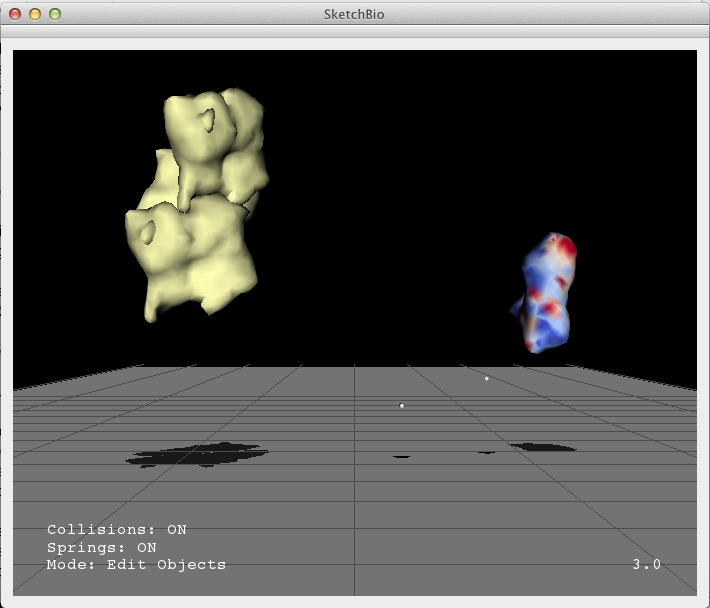
\includegraphics[width=0.8\textwidth]{actinVinculin.png}
\caption{A screen shot from SketchBio showing three actin monomers on the left colored yellow and the tail region of the vinculin protein on the right colored by surface charge.}
\label{fig:actin_vinculin}
\end{figure}

Figure \ref{fig:actin_vinculin} shows a screenshot of SketchBio's user interface with three actin molecules (left) and the tail region of a vinculin molecule (right).  The small white spheres in the center represent the two tracked hand-held controllers.  In the lower left, status information about the current state of the system is seen.  One of the main uses of SketchBio is creating animations; this project is an animation and the time in the animation is seen on the lower right in seconds.  This image also shows SketchBio coloring the objects, both solid colors like the yellow actin and according to some dataset like the vinculin tail on the right that is colored by surface charge.
\paragraph{Loading Molecules:}
SketchBio generates the molecular surfaces using UCSF Chimera\cite{pettersen2004ucsf}.  This subprocess is controlled via python scripting and a plugin was written for Chimera's python interface in order to export data from Chimera in the VTK file format.  This data includes not only the surface geometry but other data sets such as residue and chain identifier that map to a specific location on the surface and electrostatic potential on the surface.  These data sets allow the objects to be colored similar to the vinculin tail on the right.

\begin{figure}[h]
\centering
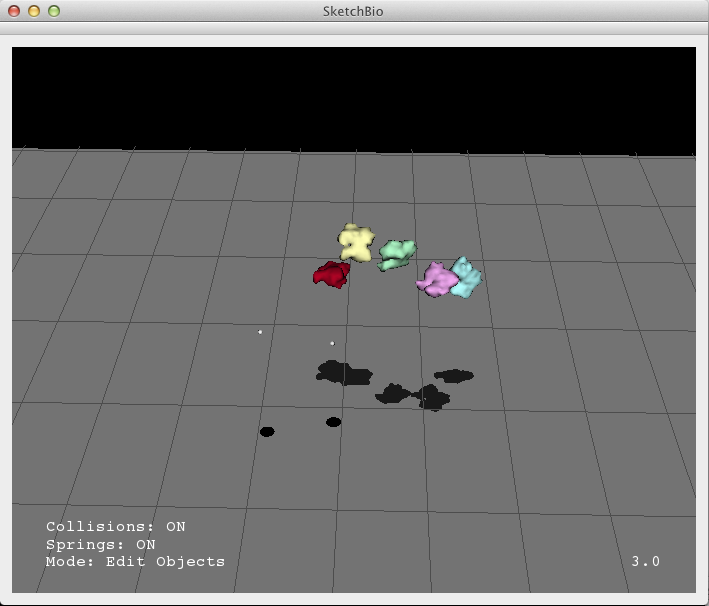
\includegraphics[width=0.8\textwidth]{shadow_plane.png}
\caption{A screenshot from SketchBio showing colored molecules and a different camera angle to emphasize the shadow plane's effect.}
\label{fig:shadow_plane}
\end{figure}
\paragraph{Shadows:}
Selection in SketchBio involves moving the tracker to a location within the bounding box of the object.  Thus, determining the relative depth between the tracker and the object is an important and often-performed task.  To provide additional depth cues, SketchBio displays a ground plane that is always rendered below the viewpoint no matter the direction or position of the viewpoint and projects the shadows of objects onto this plane.  The trackers also cast shadows onto this plane and these are darker to easily distinguish between the two.  Hendrix and Barfield found the most effective techniques for aiding in depth estimation are a textured plane and lines dropped from the center of an object to the textured plane \cite{Hendrix1995103}.  SketchBio assumes a light infinitely far away in the default camera's up direction which gives the same absolute position against the textured surface as the drop-lines while also giving information about how close the boundaries of two objects are to each other.  The user can also rotate the camera while leaving the light and shadow plane fixed to get a better understanding of the scene through motion parallax [See Figure \ref{fig:shadow_plane}].

\begin{figure}[h]
\centering
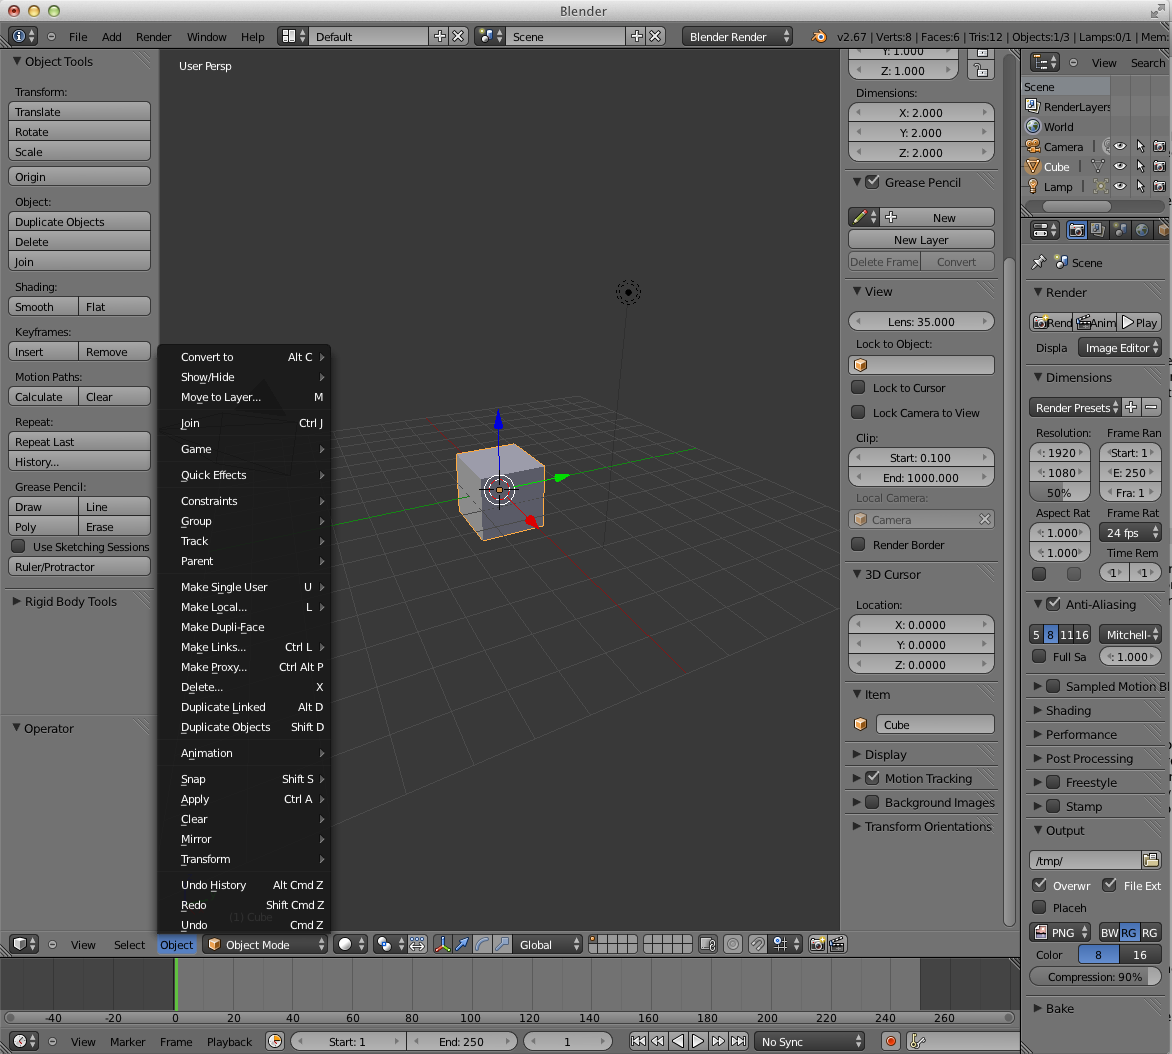
\includegraphics[width=0.8\textwidth]{blender_interface.png}
\caption{A screenshot showing the complexity of Blender's user interface.}
\label{fig:blender_interface}
\end{figure}
\paragraph{Animation:}
For scientists creating animations of molecules, SketchBio provides a basic interface to a much more complex system.  Blender is a production level animation and rendering tool.  It has an extremely complex user interface with dozens of hotkeys, menus and buttons that takes weeks or months to learn to use well (see Figure \ref{fig:blender_interface}).  Blender also has a python scripting interface that allows access to all of its functionality.  SketchBio uses Blender's python scripting interface to create its animations and render them in a high quality rendering engine, but provides a much simpler way to access that interface.  SketchBio provides simple operations, moving along the video timeline and setting keyframes on objects.  Keyframes save not only position and orientation of the objects but also other changeable aspects such as color.  This is exported to Blender with a set of global settings for effects and position of light sources to produce a full quality rendering.

\begin{figure}[h]
\centering
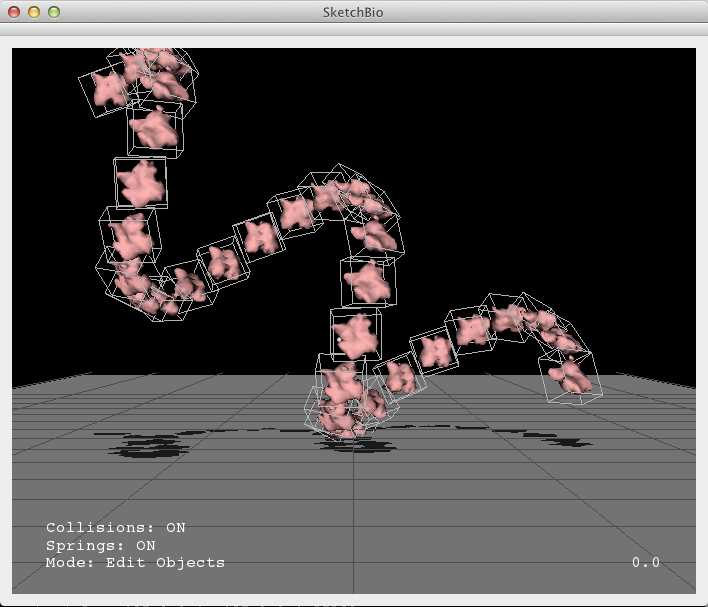
\includegraphics[width=0.8\textwidth]{crystalByExample.png}
\caption{A screenshot from SketchBio showing a contrived crystal-by-example structure that forms a helix.}
\label{fig:crystal_by_example}
\end{figure}
\paragraph{Crystal-By-Example:}
SketchBio has some features that enable quick creation of typical biological structures.  Repeated structures that are formed from a single type of protein such as the contrived helix in figure \ref{fig:crystal_by_example} are somewhat common in biology, so the ‘crystal-by-example' feature was added.  This feature allows example molecules A and B to define the entire repeated structure.  Given $T_A$ and $T_B$, the transformation matrices that define the positions of A and B relative to the world origin, the transformation from A's coordinate system to B's coordinate system, $T_{AB} = T_A^-1*T_B$, can be computed.  Then B's position can be rewritten $T_B = T_A*T_{AB}$.  This allows the creation of the next repeated molecule, C, with position $T_C = T_B*T_{AB} = T_A*T_{AB}^2$.  This can be extended to generate arbitrary numbers of molecules in a structure that is determined simply by the first two.  Many biological structures including actin fibers and microtubules form in structures that can be defined this way.  Figure \ref{fig:crystal_actin} shows an actin fiber generated this way in SketchBio.  By live updates of the entire structure as the initial two objects are manipulated, SketchBio enables the scientist to explore possibilities of these structures in real time.  Some of these structures have a known transformation from one molecule to the next.  Similar to many other programs, SketchBio also lets the user input the transformation to use between any two molecules to support more accurate construction of this kind of structure.

\begin{figure}[h]
\centering
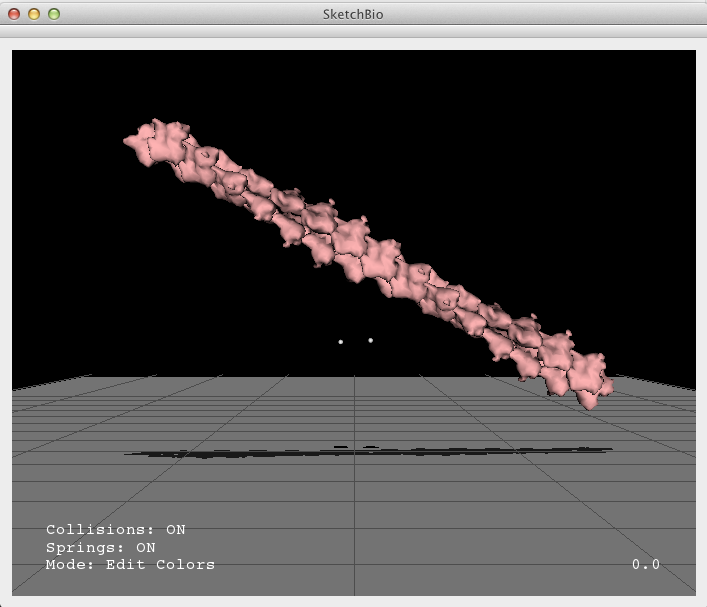
\includegraphics[width=0.8\textwidth]{crystal_actin.png}
\caption{A screenshot from SketchBio showing an actin filament created with the crystal-by-example function and using the transformation matrix from the PDB data from one monomer to the next.}
\label{fig:crystal_actin}
\end{figure}
\paragraph{Grouping:}
Grouping of molecules into larger units is also supported to make constructing larger order structures easier.  This also allows smooth animation of objects that are moving together without the small variations that even the most careful hand-placement will create.  Copy and paste is also implemented and both single objects and groups can be copied and pasted, even between sessions.
\paragraph{Connectors:}
SketchBio also has connectors that can be added between objects.  These can act like springs and apply forces to keep objects positioned relative to each other or they can simply indicate that two objects are connected.  For many proteins there are regions for which the structure is unknown and these regions can be represented with these connectors.  Because accurate molecular force calculations are not possible for large molecules at interactive rates, only very simple physics is applied and an extremely viscous fluid is assumed which negates all momentum.

\section{Simplification}

\begin{figure}[h]
	\centering
	\begin{subfigure}[b]{0.4\textwidth}
		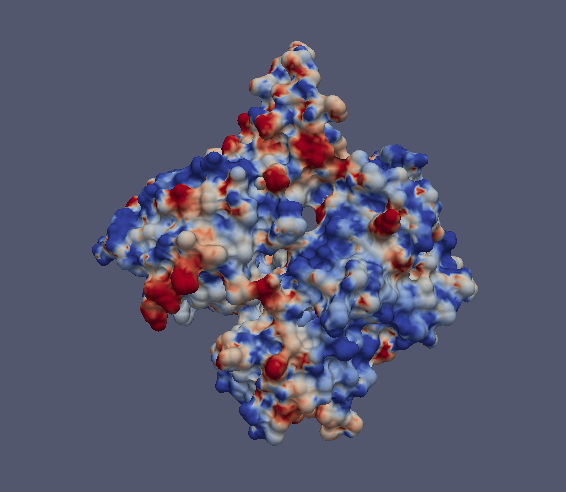
\includegraphics[width=\textwidth]{fullResolution.png}
		\caption{The full resolution surface}
		\label{fig:fullResolution}
	\end{subfigure}
	\begin{subfigure}[b]{0.4\textwidth}
		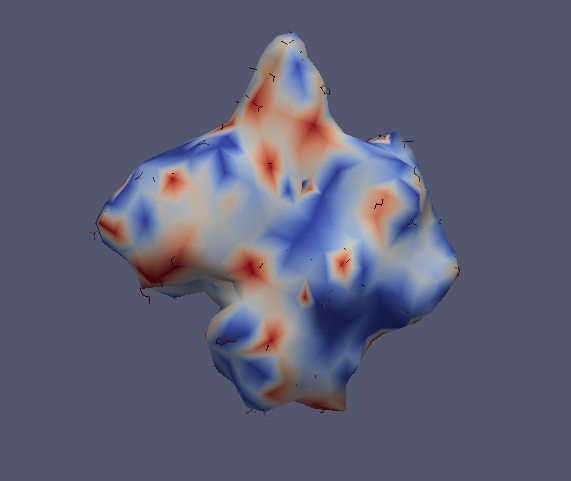
\includegraphics[width=\textwidth]{isosurface.png}
		\caption{The isosurface approximation}
		\label{fig:isosurface}
	\end{subfigure}
	\caption{Resolutions of surface produced by UCSF Chimera and used by SketchBio}
	\label{fig:resolutions}
\end{figure}

\subsection{Simplifying Geometry}
Simplifying the geometry of objects is beneficial to both collision detection and rendering times as discussed above.  There are many possible ways to accomplish this simplification.  The current implementation of SketchBio accomplishes this simplification by creating a version of each molecule's geometry at multiple resolutions. Each molecule has its full resolution surface, the Connolly solvent excluded surface for water, which is the surface used when exporting to any rendering application. This surface is shown in Figure \ref{fig:fullResolution}. Each molecule also has a simpler surface, which is generated using UCSF Chimera via an isosurface algorithm and shown in Figure \ref{fig:isosurface}. This surface is stored at its full resolution as well as a version decimated via the vtkDecimatePro filter at 5000, 2000, and 1000 triangles.  The resolution of each surface that is displayed is dependent on the number of objects that are using that geometry.

% Really not sure about this paragraph... too brutally honest?
This simplification is beneficial to the speed of the collision detection system since it guarantees that models with many copies are simple, but is less than optimal for the rendering system.  The simplification technique also lacks several guarantees that would be more optimal for the collision detection.  For convex regions of the molecule surface, the simplification algorithm guarantees that the simplified surface is inside the original surface.  However for concave regions the reverse is the case and the surface expands up to the simplification error threshold.  The algorithm guarantees that the topology of the surface is preserved, but does not make guarantees about the resulting surface being outside or inside the original.  This makes some configurations impossible without collision using simplified molecules that would be possible with no collisions using the original molecules while allowing the collision detection to run faster when there are collisions since fewer trinagles will be in collision.  Additional discussion of alternative unimplemented strategies for this is found in section \ref{sec:simplification_strategies}.

\subsection{Simplifying the Number of Collision Tests}
Improving the amount of time needed to test a pair of objects for collisions was discussed in the last section.  However, because PQP relies on statically built models and does not support merging its collision models, there is also the problem of determining which pairs of objects to test for collisions.  In the brute force solution, every object must be tested against every other object to determine if a collision has occurred.  Some response is then applied to attempt to undo the collision, but the response itself may cause other collisions which must be tested for. In a physics simulation with every object moving, every object must be checked against every other object at each timestep. This means that for a system with $n$ objects, ${n \choose 2}$ or $\mathcal{O}(n^2)$ tests must be performed at each frame.  Using spatial binning strategies or bounding volume hierarchies can reduce the complexity of the collision tests by adding much more bookkeeping on top of moving objects as discussed earlier.  But if some data about the motions of objects or their relative positions is known, the number of tests can potentially be reduced without implementing a more complex strategy.  These knowledge based simplifications could also be combined with a strategy like spatial subdivision for an even greater speedup, although this is not currently implemented.

\subsubsection{Pose Mode}
An observation about the motions of objects in SketchBio is: for most of the time working with the program, the only objects that move are those directly being manipulated by the user.  The user may even find it annoying if the object they are moving pushes the object they are attempting to dock it with away every time they accidentally collide.  Therefore one simplification that can be made to collision detection is to employ what we call pose mode physics.  In pose mode physics, only the objects directly manipulated by the user are allowed to move.  Each other object is fixed in place and does not even move due to collision response forces.  This allows an easier time docking the molecules as the molecule not being held does not get pushed away while also allowing the collision tests between the objects that the user is not interacting with to be skipped since it is known that these objects did not move.  The only way that those objects could be in collision was if they were already in collision before.  If the collision response failed to fix the collision then, it will not fix it now, so their tests can be skipped.  This means that only collisions involving the objects that the user is moving need to be checked.  This reduces the number of collision tests to $m*n$ where m is the number of objects that the user is currently moving.  The typical number of objects that the user moves at a time is 1 or a small constant in the case of moving a group, which reduces the number of collision tests needed to $\mathcal{O}(n)$ in this expected case.

\subsubsection{Crystal-by-example}
There are two ways that the user can interact with a crystal-by-example structure: moving the entire structure as a unit, or adjusting the internal transformation to change the shape of the structure.  In the first case, only collision tests between the structure and the other objects in the scene need to be done, and the above bound applies to the number of tests  Since the structure was moved as a unit, its internal geometry did not change and if there were no internal collisions to begin with, there will be none after it was moved.  In the second case, the internal structure did change and both internal and external collisions must be tested.  External collisions must test every object in the structure with every external object as above.  Let $X_i$ be the ith object in the crystal by example structure with $X_0$ and $X_1$ being the two base object in the structure.  Let $T_{i,j}$ be the transformation matrix from $X_i$ to $X_j$.  The definition of the crystal-by-example structure is that $T_{i,i+1}$ is the same for all $i$ and the geometries of all the $X_i$s are the same.  Since the geometries and transformations are the same, if there is a collision between the $ith$ and $(i+1)th$ objects anywhere in the structure, then there is also a collision between the $0th$ and $1st$ objects.  Thus testing only this one pair performs the work of n-1 tests where n is the number of objects in the structure.  This same argument holds for any $i$ and $i+k$, the $0th$ and $kth$ objects have the same relative positions and the same collisions.  Thus only the $0th$ object in the structure needs to be tested against the others which allows $\mathcal{O}(n)$ tests to suffice for all internal collisions in a repetitive structure of $n$ elements.

\section{Results}
\subsection{Model Creation}

\begin{figure}[h]
\centering
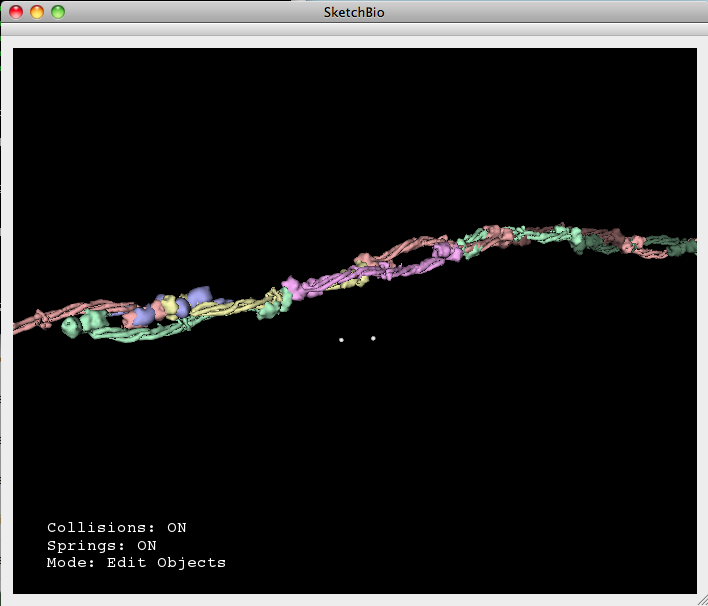
\includegraphics[width=0.8\textwidth]{joe_test.png}
\caption{A view of the model Joe Hsiao created with SketchBio to compare usibility with UCSF Chimera}
\label{fig:joe_test}
\end{figure}

Constructing the protofibril models for Susan Lord took Resource computer scientist Joe Hsiao 3-3.5 hours by hand-editing transformations within Chimera (a task challenging to teach to biologists).  Using an early prototype of SketchBio, he constructed the protofibril seen in Figure \ref{fig:joe_test} in 1.5 hours (a task we'd expect a collaborator to do just as rapidly).  From this demonstration the lack of depth cues became apparent and later the shadow plane was added.  This should reduce the amount of time needed to construct the protofibril model in SketchBio even further.

\begin{figure}[h]
\centering
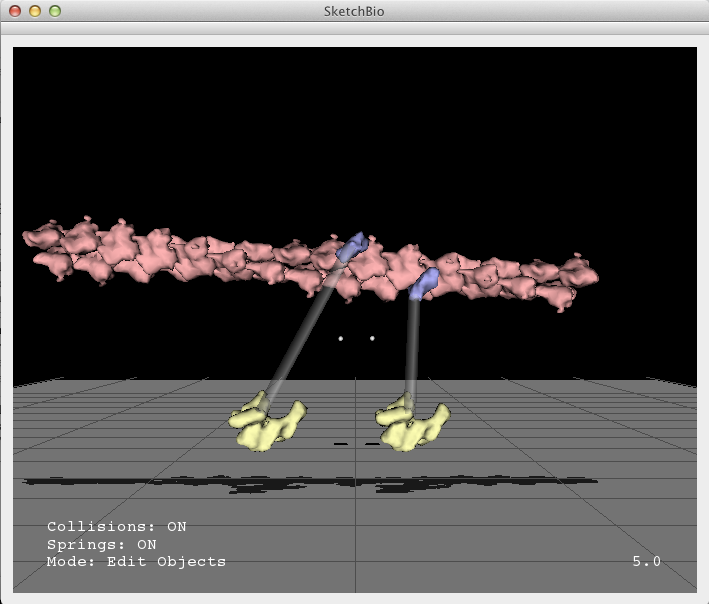
\includegraphics[width=0.8\textwidth]{peter_model.png}
\caption{A scene from a video created by Peter Thompson in SketchBio.  Approximately the same timestep is shown rendered at its full resolution in Figure \ref{fig:peter_video}}
\label{fig:peter_model}
\end{figure}


Recently, collaborator Peter Thompson, a biochemisty graduate student, created an animation of vinculin binding to an actin fiber.  The animation is based on the model presented in a recent paper.  He was able to create the video with minimal help from a computer scientist and plans to use it in an upcoming talk.  The model in SketchBio is shown in Figure \ref{fig:peter_model} and a screenshot from the resulting video at approximately the same time is shown in Figure \ref{fig:peter_video}.  Peter has said that to make a single animation, he would use Powerpoint animations to create a lower quality animation more quickly, but for making more than one animation, he thinks it is worth it to learn SketchBio.


\begin{figure}[h!]
\centering
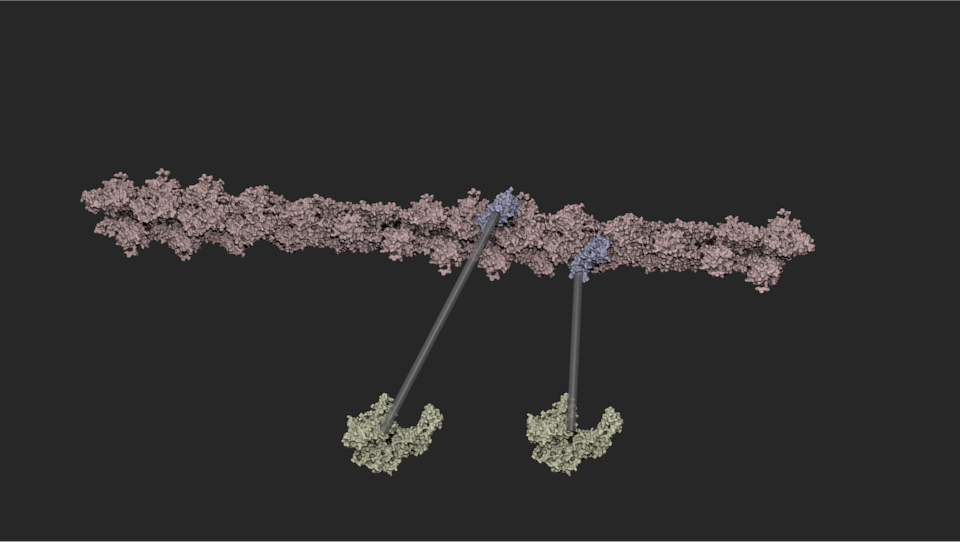
\includegraphics[width=0.8\textwidth]{peter_video.png}
\caption{A frame from the video created by Peter Thompson.  This shows the tail domains of vinculin binding to an actin filament and slowing its motion.  This video was created in SketchBio as seen in Figure \ref{fig:peter_model} and rendered via the export to Blender feature.}
\label{fig:peter_video}
\end{figure}

\subsection{Simplification}
A prototype of the collision detection simplification for crystal-by-example structures described in section 4.2 was implemented and compared against a version without the simplification.  Even with 66 copies of the object in the crystal by example structure, rendering time was so much greater than collision detection time that the timing of collision detection time was left off in order to investigate improving the rendering.  The current version can now render more than 66 moving 1000 triangle meshes interactively and over twice that many if they are not moving.

\section{Plans for Extending SketchBio}
\subsection{Utilizing Background Cores}
There are many operations which run for a long time and block the user interaction in the current implementation of SketchBio.  Several of these could be moved to background threads or subprocesses to run on any available cores while the user continues working uninterrupted.  A good example of this is surfacing and loading a molecule from the Protein Data Bank.  First UCSF Chimera is used to create a full resolution Connolly surface for the molecule.  This surface is too complex to render many copies in real time so Chimera is called again to generate a simpler isosurface based model.  Finally the surface is loaded and preprocessing is done by the collision detection library to create the bounding volume hierarchy that will be input to the collision detection functions.  This loading routine takes between 10 and 45 seconds to run depending on the complexity of the molecule being loaded.  Here I propose an alternate loading scheme that will take far less time and allow the user to work even with part of the work left undone.  The only operation that is strictly necessary for using the molecule in SketchBio is to have the simpler isosurface model of the molecule.  This operation must be blocking since the user expects the next action to be the molecule surface appearing in the SketchBio window.  However, the other two parts of the loading process can be backgrounded since they are not immediately needed.  The other Chimera job can be launched in the background to create the Connolly surface for the molecule which will not be needed until the scene is rendered at full resolution or exported to another program that needs the full resolution.  Building the bounding volume hierarchy used by collision detection from the surface data can also be done in the background since collision detection is an option that can be disabled.  The object simply won't collide with the other objects until the hierarchy has been generated.  This will allow a shorter wait for the scientist, allowing them to get more useful work done.

An additional level of complexity here is that the time to export from Chimera is highly dependent on the data that is being exported.  Adding the electrostatic potential at the surface of the object is an expensive operation and can double the import time for the model.  This leads to an optimization similar to the above: load in only what is necessary to show a molecule to the user initially and load the rest in the background.  This also allows the molecule to be surfaced quickly and returns control to the user who can perform operations while the rest of the data is being loaded.

When creating animations, it is useful to have an idea of what the final result will look like.  The background job system could be extended to render the camera's current view in the background and display it when it is done rendering.  The full-resolution rendering, which is done in Blender, cannot be done in real time, it takes several seconds to render a frame.  However, a view that shows this full resolution image can be created by using Blender in the background to render the current state of the project with a several second delay.  This will allow the user to have a better idea of what the end result of their animation will be without having to render the whole thing, which is a very long running application even for relatively short videos.

A complication when creating keyframe based animations is determining if there are collisions between keyframes.  Especially when using spline-based interpolation approaches, it becomes difficult for the user to determine just by the placement of the keyframes whether they will cause objects to pass through each other during the animation.  This is a long-running computation that could be run in a background thread and then the result displayed to the user when it finishes as it has to test for collisions at every time step over the whole animation.  This will be an heads up notificaiton to the user that there are collisions in the animation at some time.  The user can then open the notification to be taken to the time in question and shown the collision.

Another view that would be useful to the scientist is the output of the Microscope Simulator's Florosim mode.  This is currently an export option in SketchBio to allow the scientist to compare their theoretical model of the molecules in SketchBio to the output they would see if viewing this through a fluorescence microscope.  This could be done similar to the Blender animation view as a slow-to-update view of the model.  Like the full-resolution rendering view described above, this view would allow the scientist to have faster feedback about the end result of the project they are working on and potentially catch errors earlier.  This allows more useful work to be done instead of having to build the whole model and then run the simulator.

\subsection{Alternative Simplification Strategies}
\label{sec:simplification_strategies}
The current object simplification strategy in SketchBio uses precomputed simplified geometries which are replaced when the number of objects with the given geometry exceeds a threshold.  While this lowers collision detection times slightly in the case where there are many polygons overlapping, collision detection times are not currently the bottleneck of SketchBio.  The simplifications should be changed to address the current bottleneck, the rendering time.  Instead of only the number of copies of a model determining its simplification level, its distance from the screen should determine the simplification level as discussed in Luebke \cite{luebke2003level}.  Objects far from the screen should be drawn as simple textures on rectangles, objects close should be seen in full resolution and objects in the middle range can be displayed as a simplified version of the geometry.  This allows the screen size to be the determining factor in the effort of rendering.  Collision detection will still contribute to the overall time, simplifications such as discussed in section 4.2 may reduce this time enough that model simplifications are unnecessary.

When moving to larger scale models, additional simplification must be employed.  At larger scales, single molecules are only a few pixels unless they are extremely close to the camera.  Rendering even the simplified geometry for the molecules at this scale cannot be done interactively for the number of molecules needed to make an interesting scene.  This additional simplification should take advantage of overall shape information about the groups of molecules involved.  For example, an actin fiber is almost cylindrical and could be approximated as a textured cylinder.  At this zoom level, even simplifying molecules to three orthogonal textured planes will not cause a great loss of detail.  This technique or a similar one should be used for molecules that are not part of a larger structure that can be simplified in other ways.

Similar simplifications for the collision model would make it difficult for the user to dock objects, but at this scale, exact docking between molecules would be impossible anyway as it involves manipulations below the resolution of the tracker.  With many thousands of molecules in the scene, it will be necessary to combine pose mode physics with other simplification strategies such as bounding volume hierarchies or spatial bins to speed collision detection up further.  This can be done by testing each object that moved against the hierarchy or the neighboring bins to test for collisions instead of testing against all other objects as is currently implemented.

\section{Future Work}
Currently SketchBio supports exporting data to only one other tool: Blender for making animations.  But SketchBio is meant to be used as more than a quick animation creation tool.  Exporting data to simulation packages would allow it to be used as a way that a scientist with little knowledge of programming and file formats to easily specify the starting state of their simulations.  This would require keeping the atomic coordinates and/or the PDB files in addition to the surfaces generated and writing an input file to the simulator using this data.  And exporting the data to a microscope simulator would allow the model that is being built to be tested against the actual data coming in from the microscope.  This could even include positioning fluorophores by hand or automatically in SketchBio and exporting these to the simulator.  These additional exports will make SketchBio useful for new classes of tasks and provide additional opportunities for creating background jobs or new techniques.

\section{Conclusion}
The current state of SketchBio allows users to position molecules with collision detection, create repeated structures with crystal-by-example, and create animations by placing keyframes in time to specify the paths the objects take.  It has already been used by a scientist to create a video that he feels is usable in a presentation to others in his field.  This animation was based on a model from a paper he had read and wished to present.  He also created a model based on a second paper using the charge-colored surfaces to see the interaction propsed.  The developers of the tool were able to create an animation showing an approximation of the interaction between several of the molecules in about 30 minutes.  Although more work is required, this use shows that this tool is capable of letting scientists create models and animations without directly including a computer scientist or animator in the process.

\section{Acknowledgements}
This work was supported by NIH grant 5-P41-EB002025.

Molecular graphics and analyses were performed with the UCSF Chimera package. Chimera is developed by the Resource for Biocomputing, Visualization, and Informatics at the University of California, San Francisco (supported by NIGMS P41-GM103311).

% bibliography for sources used
\bibliographystyle{plain}
\bibliography{sources}

\end{document}